\documentclass[11pt]{scrartcl}
\usepackage[utf8]{inputenc}
\usepackage[croatian]{babel}
\usepackage{datetime}
\newdate{date}{13}{06}{2023}
\date{\displaydate{date}}
%\usepackage[a4paper,margin=0.5in]{geometry}
\usepackage{amsfonts}
\usepackage{amsmath}
\usepackage{amssymb}
\usepackage{amsthm}
\usepackage{csquotes}
\usepackage{tcolorbox}
\usepackage{tikz}
\usepackage{arydshln}
\pagenumbering{arabic} %gobble
\usepackage{float}
\usepackage{xcolor}
%\usepackage[dvipsnames]{xcolor}
%\usepackage{mathptmx} %times new roman?
\usepackage{breqn}
\usepackage[T1]{fontenc}
\usepackage{thmtools}
\usepackage{multirow}
\usepackage[unicode]{hyperref}

\definecolor{seagreen}{HTML}{21b2aa}
\definecolor{magenta}{HTML}{b2217f}
\definecolor{gold}{HTML}{ca9520}
\definecolor{red}{HTML}{da272f}
\definecolor{blue}{HTML}{4682b4}

\colorlet{rawsienna}{gold}

\hypersetup{
    colorlinks,
    linkcolor=magenta,
    citecolor=magenta,
    urlcolor=blue
}

%\addtokomafont{descriptionlabel}{\color{seagreen}}


\usepackage{enumitem}

\usepackage[style=numeric]{biblatex}
\addbibresource{literatura.bib}

\usepackage{pgfplots}
\pgfplotsset{compat=1.15}
\usepackage{mathrsfs}
\usetikzlibrary{arrows}
	
\usepackage[section]{placeins}
\declaretheorem{teorem}
\declaretheorem[sibling=teorem, style=plain]{lema}
\declaretheorem[style=remark, sibling=teorem]{napomena}
\declaretheorem[style=remark, sibling=teorem]{komentar}
\declaretheorem[style=definition, sibling=teorem]{definicija}
\declaretheorem[style=remark, sibling=teorem]{korolar}
\declaretheorem[style=remark, sibling=teorem]{zadatak}
\declaretheorem[style=plain, sibling=teorem]{propozicija}

\newcommand{\D}{\,\mathrm d}

\begin{document}

\title{Problemi popločavanja}
\subtitle{Drugi esej iz kolegija Matematički softver}
\author{Luka Šimek}
\date{Zagreb, \displaydate{date}}
\maketitle
%\bigskip
\tableofcontents
%\clearpage
%\pagenumbering{arabic}
%\newpage


\section{Uvod}
U najvećoj općenitosti, problemi popločavanja (eng.\ \textsl{tiling}) tiču se pokrivanja nekog konačnog geometrijskog područja manjim dijelovima, pri čemu gotovo uvijek podrazumijevamo da ti dijelovi pokrivaju cijelo područje i međusobno se ne preklapaju. Dio su kombinatorike, ali pojavljuju se i kao rekreativne zagonetke, u igrama, pa i u sva\-ko\-dnev\-nom životu.

Vrlo često, područje $R$ koje pokrivamo je dio ravnine određen pravokutnom koordinatnom rešetkom (eng.\ \textsl {lattice}), odnosno skup jediničnih kvadratića. Isto vrijedi za spomenute manje dije\-lo\-ve iz skupa s oznakom $\Sigma$ koje ćemo zvati \emph{pločice}. Najčešće se pri pokrivanju dozvoljava rotacija pločica (alternativno, u skup $\Sigma$ možemo naprosto ubaciti sve rotacije). Primjer takvog pravokutnog popločavanja vidimo u igri \emph{Tetris} (v.\ sliku~\ref{fig:tetris}) čije ćemo se $T$-pločice (ljubičasta) i $Z$-pločice (crvena) još dotaknuti kasnije. Jer imaju $4$ polja, te se pločice zovu i \emph{tetromine}, a postoje i \emph{domine}, \emph{tromine}, \emph{pentomine} itd.

\begin{figure}[h!]
    \centering
    \includegraphics[width=0.5\textwidth]{tetris.png}
    \label{fig:tetris}
    \caption{pločice u igri $\emph{Tetris}$}
\end{figure}

Sada je moguće i matematički adekvatno definirati popločavanje. Popločavanje skupa $R$ pločicama skupa $\Sigma$ je particija skupa $R$ takva da je svaki element particije dobiven translacijom (ili eventualno translacijom i rotacijom) nekog elementa skupa $\Sigma$. Pritom, ako pločice shvaćamo kao skupove jediničnih kvadratića kao objekata, riječ je o pravoj particiji. Ako na njih gledamo kao na dijelove ravnine, tada u particiji zahtijevamo samo disjunktnost interiora elemenata jer će se pločice nužno dirati u rubovima.

Osim pravokutne mreže ili rešetke, postoje i trokutasta i šesterokutna. Svejedno, često se problemi u jednoj mogu prebaciti u ekvivalentni problem u drugoj. Postoje i problemi popločavanja beskonačnih područja odnosno cijele ravnine, no to se zove \emph{parketiranje} ili \emph{teselacija}. Najčešće pitanje problema popločavanja upravo se tiče egzistencije popločavanja --- je li moguće dano područje popločati danim pločicama? To je pitanje kojim ćemo se prvenstveno baviti u ovom radu, a neka od drugih su:
\begin{itemize}
\item Koliko različitih popločavanja postoji?
\item Ako popločavanje ne postoji, koliko najmanje polja može ostati nepokriveno?
\item Koja su zajednička svojstva raznih popločavanja?
\item Koliko se najmanje pločica može staviti, a da se nakon toga više ne može staviti nijedna?
\item Postoji li popločavanje s nekim dodatnim svojstvom?
\end{itemize}

Svojevrsni vodič kroz takva pitanja možemo naći u~\cite{tilings}. Kao što je često u kombinatorici, ova pitanja su elementarna i razumljiva osobama s minimalnim matematičkim predznanjem, ali odgovori na njih zahtijevaju vrlo raznolike i netrivijalne metode rješavanja. U ovom radu vidjet ćemo razne metode odgovora na pitanje o postojanju popločavanja.

Jedan način za rješavanje takvih problema je direktni geometrijski argument. Primjerice, pitamo se može li se kvadrat popločati $Z$-pločicama.
\begin{figure}[h!]
\centering
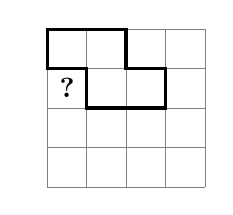
\begin{tikzpicture}
\draw[step=0.5cm,gray,very thin] (0,0) grid (4/2,4/2);
\draw[very thick] (0, 4/2) -- (0,3/2)--(1/2,3/2)--(1/2,2/2)--(3/2,2/2)--(3/2,3/2)--(2/2,3/2)--(2/2,4/2)--cycle;
\node[minimum width=1cm] at (.5/2, 2.5/2) {\textbf{?}};
\end{tikzpicture}
\caption{pokušaj popločavanja kvadrata $Z$-pločicama}
\label{slikaZ}
\end{figure}
Da pokrijemo gornji lijevi kut kvadrata, pločicu možemo postaviti jedino kao na slici~\ref{slikaZ}. No, tada je jasno da nije moguće pravilno pokriti polje označeno s \textbf{?}. Naravno, u kompliciranijim problemima neće biti ovako jednostavnih argumenata --- traženje takvog argumenta moglo bi se svesti na iscrpljivanje svih mogućih slučajeva. To je mogući pristup i pomoću računala su zaista dobiveni neki rezultati na ovom području. Ipak, i s računalom je lako moguće da takva pretraga ne bude izvediva u razumnom vremenu. Dodatno, takav način rješavanja ne pomaže u općenitijem zaključivanju. Zato nastojimo u rješavanju geometriju problema pretočiti u nešto jednostavnije. Klasični primjer toga su \emph{bojanja} kojima se bavimo u odjeljku~\ref{odj:bojanja}. To ne znači da su geometrijski argumenti uvijek nemogući ili nepotrebni (v.\ odjeljak~\ref{odj:Tplocice}).
%\newpage

\section{Neki klasični primjeri} \label{odj:bojanja}
\subsection{Bojanja}
Je li moguće popločati $7 \times 7$ ploču pločicama $1 \times 2$? Iako su oba oblika dosta pravilna, likovima površine $2$ ne možemo složiti lik površine $49$ bez preklapanja. Dakle, nužno je da površina lika dijeli površinu ploče. S druge strane, lako uspijemo popločati ploču $8 \times 8$.

\begin{zadatak} \label{sahovnicabezdva}
Sada ploči $8 \times 8$ maknemo donje lijevo i gornje desno polje. Može li se i dalje popločati pločicama $1 \times 2$?
\end{zadatak}

\begin{proof}[Rješenje]
Obojimo polja u crno i bijelo kao na šahovskoj ploči. Nakon micanja ta dva polja ostaju $32$ crna polja i $30$ bijelih polja. Svaka pločica $1 \times 2$ pokrit će jedno crno i jedno bijelo polje, stoga popločavanje nije moguće.
\end{proof}

Iako jednostavno, razmatranje površina ili šahovskog bojanja bit će od koristi u velikom broju problema. Svejedno nam često trebaju i druge ideje. U sljedećem zadatku izabrat ćemo bojanje tako da iskoristimo nesimetriju pločice.

\begin{zadatak}
Narančastu pločicu na slici~\ref{fig:tetris} zvat ćemo $L_2$-pločica. Je li moguće ploču $11 \times 4$ popločati $L_2$-pločicama?
\end{zadatak}

\begin{proof}[Rješenje]
Obojimo retke ploče naizmjence crno i bijelo kao na slici~\ref{fig:4times11}.
\begin{figure}[h!]
\centering
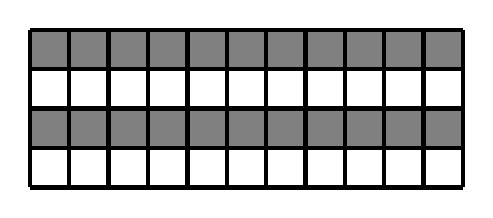
\begin{tikzpicture}
%\fill[step=1cm] (0,0) grid (11,1);
\fill[step=1cm,fill =gray] (0,1/2) rectangle (11/2,2/2);
%\fill[step=1cm] (0,2) grid (11,3);
\fill[step=1cm,fill =gray] (0,3/2) rectangle (11/2,4/2);
\draw[step = 0.5cm, ultra thick] (0,0) grid (11/2,4/2);
\end{tikzpicture}
\caption{bojanje ploče $11 \times 4$}
\label{fig:4times11}
\end{figure}
Pločica oblika $L_2$ prekrivat će ili $3$ crna polja i $1$ bijelo polje ili $1$ bijelo polje i $3$ crna polja. Pretpostavimo da se u popločavanju nalazi $m$ pločica prvog tipa i $n$ drugog tipa. Jer je ukupno $22$ polja crno i $22$ polja bijelo imamo sustav jednadžbi 
\begin{align*}
3m + n&=22\\
3n + m&=22
\end{align*}
koji nema cjelobrojnih rješenja.
\end{proof}

Sljedeći zadatak zapravo nije o popločavanju, ali opet ćemo intuicijom doći do korisnog bojanja.
\begin{zadatak}
Dana je ploča $5 \times 7$ i $L_1$-pločica (v.\ sliku~\ref{fig:L_1}).

\begin{figure}[h!]
\centering
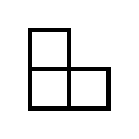
\begin{tikzpicture}

\draw[ultra thick] (0,0) rectangle (1/2,1/2);
\draw[ultra thick] (0,1/2) rectangle (1/2,2/2);
\draw[ultra thick] (1/2,0) rectangle (2/2,1/2);

\end{tikzpicture}
\caption{$L_1$-pločica}
\label{fig:L_1}
\end{figure}

\noindent Na ploču smijemo stavljati $L_1$ pločice, čak i ako se pritom preklapaju. Je li ih moguće postaviti tako da je svako polje pokriveno barem jednom, i tako da je svako polje pokriveno jednak broj puta?
\end{zadatak}
\begin{proof}[Rješenje]
Obojimo ploču kao na slici~\ref{fig:5times7}. Pločica oblika $L_1$ može pokriti ili jedno ili nijedno crno polje. Neka je pločica prvog tipa $C$, a drugog $D$. Obzirom da je svako polje pokriveno jednakim brojem pločica, posebice je jednaka aritmetička sredina tih brojeva na crnom i na bijelom području. Na crnom ona iznosi $\frac{1}{16} C$, a na bijelom $\frac{1}{19} \left(2C + 3D\right)$. Kako je $\frac{2}{19} > \frac{1}{16}$ i $C, D > 0$, jednakost tih dvaju izraza nije moguća.
\begin{figure}[h]
\centering
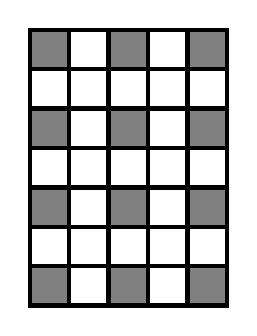
\begin{tikzpicture}
\draw[ultra thick, step = 0.5cm, draw = black] (0,0) grid (5/2,7/2);

\foreach \x in {0,2/2,4/2}{
\foreach \y in {0,2/2,4/2,6/2}
{
\draw[fill = gray, draw = black, ultra thick] (\x,\y) rectangle (\x+1/2,\y+1/2);
}}
\end{tikzpicture}
\caption{bojanje $5 \times 7$ ploče}
\label{fig:5times7}
\end{figure}
\end{proof}
\subsection{Generalizacije}
Osim bojanja koriste se i svojevrsne generalizacije. Razmotrimo težinske funkcije koje svakom polju pridružuju određenu vrijednost. Težinu nekog područja definiramo kao zbroj težina polja kojih ga čine. Ako je $w$ težinska funkcija, a $S_1, \ldots, S_n \in \Sigma$ pločice (zapravo translacije pločica iz $\Sigma$) kojima smo pokrili područje $R$, jasno je da mora vrijediti
\begin{equation}\label{tezinska}
w(R) = \sum_{i = 1}^n w(S_i).
\end{equation}
Kažemo da je u pitanju generalizacija jer na naše početno razmatranje površine možemo gledati kao na težinsku funkciju $w \equiv 1$. Šahovsko bojanje odgovara funkciji koja crnim poljima pridruži formalni polinom $x$, a bijelima $1$. Tada je težina područja polinom prvog stupnja čiji je slobodni koeficijent broj bijelih, a nagib broj crnih polja u njemu. Iako ovo može biti zanimljivo, ne doprinosi smislu niti moći ideje. Zanimljivije je primjerice crnim poljima pridružiti $1$, a bijelima $-1$. Tada je težina nekog područja razlika broja crnih i bijelih polja, što se smisleno razlikuje od ostaloga. Sljedeći zadatak pojavit će se kao korolar teorema~\ref{2:teorem}, a ovdje ćemo tvrdnju dokazati i na drugi način.

\begin{zadatak}
Pravokutnik dimenzija $a \times b$ može se popločati dominama $1 \times n$ ako i samo ako $n \mid a$ ili $n \mid b$.
\end{zadatak}
\begin{proof}[Rješenje]
Neka je $\omega \neq 1$ $n$-ti korijen jedinice, dakle vrijedi $1 + \omega +\omega^2 + \dotsb + \omega^{n-1} = 0$. Nekom kutnom polju damo težinu $1$, njegovim susjedima $\omega$, zatim njegovim $\omega^2$ itd.\ do susjeda od $\omega^{n-1}$ kojima dajemo težinu $\omega^n = 1$. Težina svake pločice $1 \times n$ bit će $0$, no lako se uvjeriti da će težina cijele ploče biti $0$ ako i samo ako $n \mid a$ ili $n \mid b$.
\end{proof}
\begin{napomena}
Iako elegantno, suštinski isto rješenje dalo se provesti bojanjem u $n$ boja ili zamjenom $1, \omega, \ldots, \omega^{n-1}$ s bilo kojom drugom $n$-torkom čija je suma $0$.
\end{napomena}

Moguće je generalizirati i dalje. Obzirom da se na $R$ i pločice iz $\Sigma$ može gledati kao na podskupove $\mathbb{R}^2$, možemo definirati funkciju
\begin{align*}
f &\colon \mathbb{R}^2 \to \mathbb{R} \quad \text{ili}\\
f &\colon \mathbb{R}^2 \to \mathbb{C},
\end{align*}
a težinu nekog (izmjerivog) područja $S$ definirati kao
$w(S) = \iint_S f \D x \D y$.
Kako su integrali aditivni, vrijedit će jednakost analogna~\eqref{tezinska}:
\[
\iint_R f \D x \D y = \sum_{i=1}^n \iint_{S_i} f \D x \D y.
\]
Primjenu ove ideje vidjet ćemo u dokazu teorema~\ref{2:teorem}.
\subsection{Indukcija}
Za kraj ovog odjeljka riješit ćemo zadatak koji pokazuje raznolikost i u primjeni matematičke indukcije, i u rješavanju problema popločavanja.

\begin{zadatak} Iz ploče dimenzija $2^n \times 2^n$ maknemo bilo koje polje. Dokažite da se takva krnja ploča može pokriti $L_1$-pločicama.
\end{zadatak}

\begin{proof}[Rješenje]
Tvrdnju dokazujemo matematičkom indukcijom. Bazni slučaj $n = 2$ je trivijalan. Pretpostavimo da tvrdnja vrijedi za neki $n \in \mathbb{N}$. Dokažimo da tada tvrdnja vrijedi i za $n+1$. Proizvoljnu krnju ploču dimenzija $2^{n+1} \times 2^{n+1}$ podijelit ćemo na $4$ ploče dimenzija $2^n \times 2^n$.
\begin{figure}[h!]
\centering
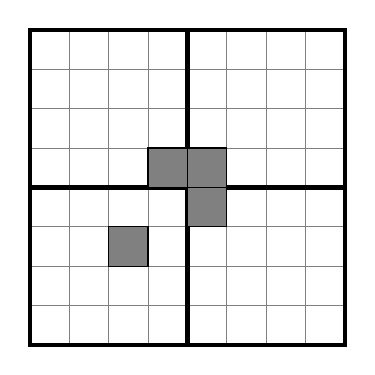
\begin{tikzpicture}
\draw[very thin, step = 0.5cm, draw = gray] (0,0) grid (4,4);
\draw[ultra thick] (0,2)--(4,2);
\draw[ultra thick] (2,0) -- (2,4);
\draw[ultra thick] (0,0) -- (0,4) -- (4, 4) -- (4,0) -- cycle;

\draw[fill = gray] (1, 1) rectangle (1.5,1.5);
\draw[fill = gray] (2, 1.5) rectangle (2.5,2);
\draw[fill = gray] (2, 2) rectangle (2.5,2.5);
\draw[fill = gray] (1.5, 2) rectangle (2,2.5);
\end{tikzpicture}
\caption{primjer za $n + 1= 3$}
\label{fig:indukcija}
\end{figure}
Bez smanjenja općenitosti možemo pretpostaviti da se maknuto polje nalazi u donjem lijevom dijelu ploče. I ostale tri ploče pretvorimo u krnje ploče tako da im maknemo polja u obliku $L_1$-pločice (v.\ sliku~\ref{fig:indukcija}). Sada se sve manje ploče mogu pokriti $L_1$-pločicama po prepostavki indukcije, dok se tri dodatno maknuta polja pokriju jednom dodatnom $L_1$-pločicom.
\end{proof}
%\newpage

\section{Popločavanje pravokutnika pravokutnicima}
Jedan od najjednostavnijih i najpraktičnijih problema popločavanja je popločavanje većeg pravokutnika manjima. Pitamo se pod kojim je uvjetima moguće pravokutnik dimenzija $m \times n$ popločati pravokutnicima dimenzija $a \times b$. Primjerice, jasno je da je popločavanje moguće kada $a \mid m$ i $b \mid n$, ali je li to i nužno? Odgovor je ne --- i riječ je o riješenom problemu. Nužni i dovoljni uvjet daje sljedeći teorem.

\begin{teorem} \label{2:teorem}
Pravokutnik dimenzija $m \times n$ može se popločati pravokutnicima dimenzija $a \times b$ ako i samo ako vrijede sljedeća tri uvjeta:
\begin{itemize}
\item $ab \mid mn$,
\item $m$ i $n$ se mogu prikazati kao suma (pozitivnog broja) pribrojnika $a$ i $b$,
\item $a \mid m$ ili $a \mid n$, a također i $b \mid m$ ili $b \mid n$.
\end{itemize}
\end{teorem}

\begin{proof}
Prvo dokažimo da su uvjeti nužni. Nužnost prvog uvjeta je očita. Za drugi uvjet, gledajmo rub velikog pravokutnika duljine $m$. Prilikom popločavanja on će biti pokriven rubovima manjih pravokutnika, svaki od kojih je duljine $a$ ili $b$. Dakle, $m$ mora biti prikaziv kao zbroj više pribrojnika jednakih $a$ ili $b$. Isto vrijedi za rub duljine $n$.

Posvetimo se sada trećem uvjetu. Najprije, lako se uvjeriti da je
\[
\int _\alpha ^\beta \sin 2 \pi x \D x= 0
\]
ako i samo ako je $\alpha + \beta$ ili $\alpha - \beta$ cijeli broj. Korolar toga je da
\[
\frac 1a \int _\alpha ^\beta \sin 2 \pi a x \D x = \int _{\alpha/a}^{\beta/a} \sin 2 \pi x \D x = 0
\]
vrijedi ako i samo ako $a \mid \alpha - \beta$ ili $a \mid \alpha + \beta$. Sada ćemo na pravokutnike gledati kao na konkretne podskupove $\mathbb{R}^2$. Po gornjoj tvrdnji za svaki mali pravokutnik $S$ vrijedi
\[
\iint _S \sin 2 \pi ax \sin 2 \pi ay \D x \D y = 0
\]
jer ima ili horizontalnu ili vertikalnu stranicu jednaku $a$. Zbog aditivnosti integrala, ista funkcija poništit će i integral na velikom pravokutniku $R$, dakle
\[
\iint _R \sin 2 \pi ax \sin 2 \pi ay \D x \D y = 0
\]
iz čega slijedi da $a \mid m$ ili $a \mid n$. Analogno se dokaže tvrdnja za $b$.

Dokažimo i da su uvjeti dovoljni. Lako je naći popločavanje u slučaju da $a \mid m$ i $b \mid n$. U gornjem lijevom kutu velikog pravokutnika položimo mali tako da rub duljine $a$ leži uz rub duljine $m$ te u istom smjeru nanižemo mogućih $m/a$ malih pravokutnika. Ponavljanjem postupka $n/b$ puta popločat ćemo cijeli veliki pravokutnik. Preostaje slučaj kada $a \mid m$ i $b \mid m$. Pretpostavimo još da je $n = ak + bl$, $k, l \in \mathbb{N}$. Kao u prošlom slučaju, počnimo polagati male pravokutnike tako da rub duljine $a$ leži uz rub duljine $m$ i ponovimo postupak $k$ puta. Ostaje nam za pokriti pravokutnik dimenzija $m \times ak$ čime smo došli do prethodnog slučaja. Primjer popločavanja u drugom slučaju dan je na slici~\ref{fig:6723}.
\end{proof}

\begin{figure}[ht]
\centering
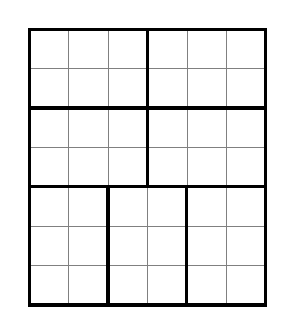
\begin{tikzpicture}
\draw[step=0.5cm,gray,very thin] (0,0) grid (6/2,7/2);
\draw[very thick] (0,0) rectangle (2/2,3/2);
\draw[very thick] (2/2,0) rectangle (4/2,3/2);
\draw[very thick] (4/2,0) rectangle (6/2,3/2);
\draw[very thick] (0,3/2) rectangle (3/2,5/2);
\draw[very thick] (3/2,3/2) rectangle (6/2,5/2);
\draw[very thick] (0,5/2) rectangle (3/2,7/2);
\draw[very thick] (3/2,5/2) rectangle (6/2,7/2);
\end{tikzpicture}
\caption{popločavanje pravokutnika $6 \times 7$ pravokutnicima $2 \times 3$}
\label{fig:6723}
\end{figure}

\begin{komentar}
Najzanimljiviji dio dokaza je nužnost trećeg uvjeta. U~\cite{wagon} može se naći $14$ dokaza malo općenitije tvrdnje.
\end{komentar}

\begin{korolar} \label{2:korolar}
Pravokutnik dimenzija $a \times b$ može se popločati dominama $1 \times n$ ako i samo ako $n \mid a$ ili $n \mid b$.
\end{korolar}
\subsection{Osvrt na \texorpdfstring{$L_1$-pločice}{TEXT}}

Pomoću dvije $L_1$-pločice (v.\ sliku~\ref{fig:L_1}) može se složiti $2 \times 3$ pravokutnik. Iz teorema~\ref{2:teorem} slijedi da se pravokutnik dimenzija $3m \times n$ može popločati $L_1$-pločicama čim je
\begin{itemize}
\item $n$ paran ili
\item $m$ paran i $n \geq 2$.
\end{itemize}
To ipak nisu svi pravokutnici koji se mogu pokriti $L_1$-pločicama. 
\begin{lema} \label{L_1:lema}
Pravokutnik dimenzija $9 \times 5$ može se popločati $L_1$-pločicama.
\end{lema}
\begin{proof}
Primjer je dan slikom~\ref{fig:9times5}.
\begin{figure}[ht]
\centering
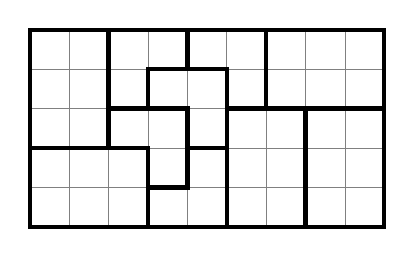
\begin{tikzpicture}
\draw[step=0.5cm,gray,very thin] (0,0) grid (9/2,5/2);
\draw[ultra thick] (0,0) rectangle (3/2, 2/2);
\draw[ultra thick] (0, 2/2) rectangle (2/2, 5/2);
\draw[ultra thick] (6/2, 3/2) rectangle (9/2, 5/2);
\draw[ultra thick] (5/2, 0) rectangle (7/2, 3/2);
\draw[ultra thick] (7/2, 0) rectangle (9/2, 3/2);
\draw[ultra thick] (2/2, 5/2) -- (2/2, 3/2) -- (3/2,3/2)--(3/2,4/2)--(4/2,4/2) -- (4/2,5/2) -- cycle;
\draw[ultra thick] (6/2,5/2)--(4/2,5/2)--(4/2,4/2)--(5/2,4/2)--(5/2,3/2);
\draw[ultra thick] (3/2,3/2)--(4/2,3/2)--(4/2,2/2)--(5/2,2/2);
\draw[ultra thick] (4/2,2/2)--(4/2,1/2)--(3/2,1/2); \draw[ultra thick](3/2,0)--(5/2,0);
\end{tikzpicture}
\caption{popločavanje pravokutnika $9 \times 5$ $L_1$-pločicama}
\label{fig:9times5}
\end{figure}
\end{proof}
\noindent Ta činjenica uvelike povećava skup pravokutnika kojih se može popločati $L_1$-pločicama.
\begin{teorem} Pravokutnik dimenzija $3m \times n$ može se popločati $L_1$-pločicama ako i samo ako vrijedi jedan od sljedećih uvjeta:
\begin{itemize}
\item $m = 1$ i $n$ je paran,
\item $m$ je paran i $n \geq 2$ ili
\item $m \geq 3$ je neparan i $n \neq 1,3$.
\end{itemize}
\end{teorem}
\begin{proof}
Neka su $m \geq 3$ i $n \geq 5$ neparni. Dokažimo da se pravokutnik dimenzija $3m \times n$ može pokriti $L_1$-pločicama. Ostali slučajevi pokriveni su teoremom~\ref{2:teorem}. Razlikujemo nekoliko slučajeva:
\begin{itemize}
\item $3m \equiv 0 \pmod{9}$. Pokrijemo gornji lijevi $9 \times 5$ pravokutnik tako da rub duljine $9$ leži uz rub duljine $3m$. Ponovimo to $3m/9$ puta. Nakon toga nam ostaje za popločati (moguće degenerirani za $n=5$) pravokutnik $3m \times (n-5)$. Kako je $n - 5$ paran broj, taj se ostatak može popločati po teoremu~\ref{2:teorem}.

\item $3m \equiv 6 \pmod{9}$. Dok možemo postupamo kao u prethodnom slučaju. Zatim nam ostaje područje koje možemo podijeliti na pravokutnike $6 \times 5$ i $3m \times (n-5)$ i oba možemo popločati.

\item $3m \equiv 3 \pmod{9}$. U ovom slučaju prvo popločamo lijevi $6 \times n$ pravokutnik. Ostaje nam za popločati pravokutnik $(3m-6) \times n$. Kako je $3m - 6 \equiv 6 \pmod{9}$, ovaj smo slučaj sveli na prethodni.
\end{itemize}

Sada dokažimo nužnost uvjeta. Dokazat ćemo samo za prvi uvjet jer se ostalo vidi trivijalno. Dokazujemo, dakle, da se pravokutnik $3 \times (2k+1)$ ne može popločati $L_1$-plo\-či\-ca\-ma. Obojimo pravokutnik kao na slici~\ref{fig:5times7} --- tada imamo $2(k+1)$ crnih polja. Svaka $L_1$-pločica pokrit će najviše jedno od njih, dakle za popločavanje nam treba barem $2(k+1)$ $L_1$-pločica. Njihova bi ukupna površina bila $6k + 6$, no to je veće od površine cijelog pravokutnika koja iznosi $6k+ 3$.
\end{proof}
Ovime smo za \enquote{gotovo sve} pravokutnike čija je površina djeljiva s $3$ dokazali da se daju popločati $L_1$-pločicama. Osim osnovnog zahtjeva da je površina djeljiva s $3$, dovoljni uvjet je primjerice da su stranice pravokutnika dulje od $6$. To ne mora biti kraj proučavanja $L_1$-pločica --- primjerice su u~\cite{Ltromine} dani neki rezultati o popločavanju krnjih pravokutnika.
%\newpage

\section{Popločavanje \texorpdfstring{$T$-pločicama}{TEXT}} \label{odj:Tplocice}
Postoji lijepo popločavanje kvadrata $4 \times 4$ $T$-pločicama (ljubičasta, slika~\ref{fig:tetris}) dano na slici~\ref{fig:4times4}.

\begin{figure}[ht]
\centering
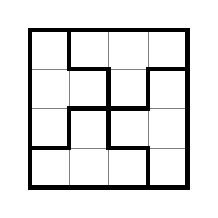
\begin{tikzpicture}
\draw[step=0.5cm,gray,very thin] (0,0) grid (2,2);
\draw[ultra thick] (0,0)--(2,0)--(2,2)--(0,2)--cycle;
\draw[ultra thick] (.5,2)--(.5,1.5)--(1,1.5)--(1,1)--(.5,1)--(.5,.5)--(0,.5);
\draw[ultra thick] (1.5,0)--(1.5,.5)--(1,.5)--(1,1)--(1.5,1)--(1.5,1.5)--(2,1.5);

\end{tikzpicture}
\caption{popločavanje pravokutnika $4 \times 4$ $T$-pločicama}
\label{fig:4times4}
\end{figure}

\noindent Odmah slijedi da se i svaki pravokutnik $4m \times 4n$ može popločati $T$-pločicama. Prirodno se pitamo je li djelivost duljina stranica s $4$ i nužni uvjet. Odgovor je potvrdan, ali dokaz je netrivijalan i zahtijeva proučavanje geometrije takvih popločavanja. Dokaz je dan u~\cite{walkup} te ćemo ga parafrazirati i ovdje.
\begin{definicija} Najprije definiramo nekoliko bitnih pojmova.
\begin{enumerate}
\item \emph{Segment} će ovdje biti dužina duljine $1$ koja je dio koordinatne rešetke.
\item \emph{Rezni segment} je segment koji se u svakoj teselaciji kvadranta između pozitivnih dijelova koordinatnih osi nalazi kao dio ruba neke $T$-pločice.
\item \emph{Ravna točka} je ona koja se ni u kojoj teselaciji ne nalazi kao vrh $T$-pločice (kao mnogokuta).
\item \emph{Translat} točke $(x,y)$ je bilo koja točka $(x + 2k, y - 2k)$ gdje je $k \in \mathbb{Z}$; time definiramo i translate drugih objekata.
\item $A$\emph{-točka} ili \emph{točka vrste} $A$ je ona čije su koordinate kongruentne $(0,0)$ ili $(2,2)$ modulo $4$, dok je $B$\emph{-točka} ona čije su koordinate kongruentne $(0,2)$ ili $(2,0)$ modulo $4$.
\end{enumerate}
\end{definicija}

\noindent Primijetimo da translat točke vrste $A$ ili $B$ ostaje točka redom vrste $A$ ili $B$ te da su svi segmenti na koordinatnim osima nužno rezni. Za dokaz bit će presudna sljedeća lema. Argumenti su prikazani pomoću slika~\ref{fig:Tlema1} i~\ref{fig:Tlema2}, ali analogno se prenose i na sve druge situacije.

\begin{lema} \label{Tlema}
Svaka $B$-točka je ravna i svaki segment koji sadrži $A$-točku je rezni segment.
\end{lema}

\begin{proof}
Tvrdnju ćemo dokazati induktivno. Tvrdimo da za svaki $k \geq 0$ tvrdnja vrijedi za sve točke na pravcu ili ispod pravca $x + y = 4k$. Baza indukcije bit će $k = 0$ --- u tom slučaju govorimo o samo dva segmenta pri ishodištu koji su očito rezni. Pretpostavimo da tvrdnja vrijedi za neki $k$ i dokazujemo da vrijedi i za $k+ 1$. 
\begin{figure}[ht]
\centering
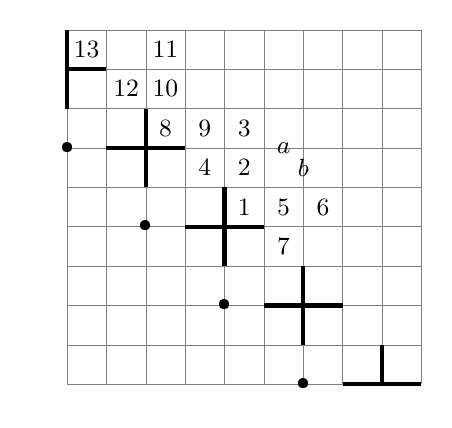
\begin{tikzpicture}
\draw[step=0.5cm,gray,very thin] (0,0) grid (9/2,9/2);
\draw[ultra thick]  (0, 7/2)--(0, 9/2);
\draw[ultra thick]  (2/2, 5/2)--(2/2, 7/2);
\draw[ultra thick]  (4/2, 3/2)--(4/2, 5/2);
\draw[ultra thick]  (6/2, 1/2)--(6/2, 3/2);
\draw[ultra thick]  (8/2, 0)--(8/2, 1/2);

\draw[ultra thick]  (0, 8/2)--(1/2, 8/2);
\draw[ultra thick]  (1/2, 6/2)--(3/2, 6/2);
\draw[ultra thick]  (3/2, 4/2)--(5/2, 4/2);
\draw[ultra thick]  (5/2, 2/2)--(7/2, 2/2);
\draw[ultra thick]  (7/2, 0)--(9/2, 0);

\node[minimum width=1cm] at (0,6/2) {\textbullet};
\node[minimum width=1cm] at (2/2,4/2) {\textbullet};
\node[minimum width=1cm] at (4/2,2/2) {\textbullet};
\node[minimum width=1cm] at (6/2,0) {\textbullet};

\node[minimum width=1cm] at (5/2+1/4,6/2) {\small $a$};
\node[minimum width=1cm] at (6/2,5/2+1/4) {\small $b$};

\node[minimum width=1cm] at (4/2+1/4,4/2+1/4) {\small $1$};
\node[minimum width=1cm] at (4/2+1/4,5/2+1/4) {\small $2$};
\node[minimum width=1cm] at (4/2+1/4,6/2+1/4) {\small $3$};
\node[minimum width=1cm] at (3/2+1/4,5/2+1/4) {\small $4$};
\node[minimum width=1cm] at (5/2+1/4,4/2+1/4) {\small $5$};
\node[minimum width=1cm] at (6/2+1/4,4/2+1/4) {\small $6$};
\node[minimum width=1cm] at (5/2+1/4,3/2+1/4) {\small $7$};
\node[minimum width=1cm] at (2/2+1/4,6/2+1/4) {\small $8$};
\node[minimum width=1cm] at (3/2+1/4,6/2+1/4) {\small $9$};
\node[minimum width=1cm] at (2/2+1/4,7/2+1/4) {\small $10$};
\node[minimum width=1cm] at (2/2+1/4,8/2+1/4) {\small $11$};
\node[minimum width=1cm] at (1/2+1/4,7/2+1/4) {\small $12$};
\node[minimum width=1cm] at (0/2+1/4,8/2+1/4) {\small $13$};
\end{tikzpicture}
\caption{situacija za $k = 2$, prvi dio}
\label{fig:Tlema1}
\end{figure}
Na slici~\ref{fig:Tlema1} prikazani su (neki) rubovi koji su rezni po pretpostavci indukcije i točke vrste $B$ u slučaju $k = 2$. Kad bi teselacija sadržavala pločicu $1/2/3/4$, jedini način da se mogu pokriti polja $8$ i $9$ je da sadrži i pločicu $8/10/11/12$. Analogno se pokaže i za sve druge translate. Zbog udaljenosti od osi $y$, nije moguće da teselacija sadrži sve translate --- očito je tada nemoguće pokriti polje $13$. Dakle, teselacija ne može sadržavati pločicu $1/2/3/4$. Postoji još četiri mogućnosti za pločicu koja pokriva $1$ i poštuje istaknute rezne segmente. Svaka od njih sadrži segment $a$ kao rub pločice, stoga je on rezni segment. Analognom argumentacijom po pločici $1/5/6/7$ pokazuje se da je i $b$ rezni segment. Također, i translati segmenata $a$ i $b$ su rezni.

\begin{figure}[h!]
\centering
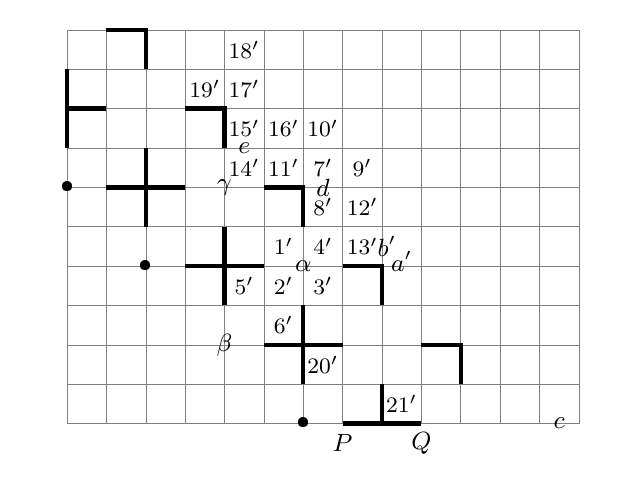
\begin{tikzpicture}
\draw[step=0.5cm,gray,very thin] (0,0) grid (13/2,10/2);
\draw[ultra thick]  (0, 7/2)--(0, 9/2);
\draw[ultra thick]  (2/2, 5/2)--(2/2, 7/2);
\draw[ultra thick]  (4/2, 3/2)--(4/2, 5/2);
\draw[ultra thick]  (6/2, 1/2)--(6/2, 3/2);
\draw[ultra thick]  (8/2, 0)--(8/2, 1/2);

\draw[ultra thick]  (0, 8/2)--(1/2, 8/2);
\draw[ultra thick]  (1/2, 6/2)--(3/2, 6/2);
\draw[ultra thick]  (3/2, 4/2)--(5/2, 4/2);
\draw[ultra thick]  (5/2, 2/2)--(7/2, 2/2);
\draw[ultra thick]  (7/2, 0)--(9/2, 0);

\node[minimum width=1cm] at (0,6/2) {\textbullet};
\node[minimum width=1cm] at (2/2,4/2) {\textbullet};
\node[minimum width=1cm] at (4/2,2/2) {\small $\beta$};
\node[minimum width=1cm] at (6/2,0) {\textbullet};
\node[minimum width=1cm] at (4/2,6/2) {\small $\gamma$};
\node[minimum width=1cm] at (7/2,-.25) {\small $P$};
\node[minimum width=1cm] at (9/2,-.25) {\small $Q$};

\draw[ultra thick] (1/2,10/2)--(2/2,10/2)--(2/2,9/2);
\draw[ultra thick] (3/2,8/2)--(4/2,8/2)--(4/2,7/2);
\draw[ultra thick] (5/2,6/2)--(6/2,6/2)--(6/2,5/2);
\draw[ultra thick] (7/2,4/2)--(8/2,4/2)--(8/2,3/2);
\draw[ultra thick] (9/2,2/2)--(10/2,2/2)--(10/2,1/2);

\node[minimum width=1cm] at (8/2+1/4,4/2+1/16) {\small $a'$};
\node[minimum width=1cm] at (8/2+1/16,4/2+1/4) {\small $b'$};
\node[minimum width=1cm] at (12/2+1/4,0) {\small $c$};
\node[minimum width=1cm] at (6/2+1/4,6/2) {\small $d$};
\node[minimum width=1cm] at (4/2+1/4,7/2) {\small $e$};

\node[minimum width=1cm] at (6/2,4/2) {\small $\alpha$};

\node[minimum width=1cm] at (5/2+1/4,4/2+1/4) {\footnotesize $1'$};
\node[minimum width=1cm] at (5/2+1/4,3/2+1/4) {\footnotesize $2'$};
\node[minimum width=1cm] at (6/2+1/4,3/2+1/4) {\footnotesize $3'$};
\node[minimum width=1cm] at (6/2+1/4,4/2+1/4) {\footnotesize $4'$};
\node[minimum width=1cm] at (4/2+1/4,3/2+1/4) {\footnotesize $5'$};
\node[minimum width=1cm] at (5/2+1/4,2/2+1/4) {\footnotesize $6'$};
\node[minimum width=1cm] at (6/2+1/4,6/2+1/4) {\footnotesize $7'$};
\node[minimum width=1cm] at (6/2+1/4,5/2+1/4) {\footnotesize $8'$};
\node[minimum width=1cm] at (7/2+1/4,6/2+1/4) {\footnotesize $9'$};
\node[minimum width=1cm] at (6/2+1/4,7/2+1/4) {\footnotesize $10'$};
\node[minimum width=1cm] at (5/2+1/4,6/2+1/4) {\footnotesize $11'$};
\node[minimum width=1cm] at (7/2+1/4,5/2+1/4) {\footnotesize $12'$};
\node[minimum width=1cm] at (7/2+1/4,4/2+1/4) {\footnotesize $13'$};
\node[minimum width=1cm] at (4/2+1/4,6/2+1/4) {\footnotesize $14'$};
\node[minimum width=1cm] at (4/2+1/4,7/2+1/4) {\footnotesize $15'$};
\node[minimum width=1cm] at (5/2+1/4,7/2+1/4) {\footnotesize $16'$};
\node[minimum width=1cm] at (4/2+1/4,8/2+1/4) {\footnotesize $17'$};
\node[minimum width=1cm] at (4/2+1/4,9/2+1/4) {\footnotesize $18'$};
\node[minimum width=1cm] at (3/2+1/4,8/2+1/4) {\footnotesize $19'$};
\node[minimum width=1cm] at (6/2+1/4,1/2+1/4) {\footnotesize $20'$};
\node[minimum width=1cm] at (8/2+1/4,0/2+1/4) {\footnotesize $21'$};
\end{tikzpicture}
\caption{situacija za $k = 2$, drugi dio}
\label{fig:Tlema2}
\end{figure}

Na slici~\ref{fig:Tlema2} dodani su novi poznati rezni segmenti i uvedene nove oznake. Dokazat ćemo da je točka $\alpha$ ravna i da su segmenti $a'$ i $b'$ rezni. Opet, to ćemo učiniti bez smanjenja općenitosti pa ćemo time završiti korak indukcije i dokazati lemu.

Pretpostavimo da $\alpha$ nije ravna točka, odnosno da je vrh neke pločice koja je dio teselacije. Jedine pločice koje poštuju rezne segmente su $1'/2'/3'/5'$ i $1'/2'/3'/6'$, no tada će biti redom nemoguće pokriti polja $6'$ ili $5'$ poštujući to da je točka $\beta$ ravna. Dakle, i $\alpha$ je ravna.

Sada dokažimo da je $a'$ rezni segment. Zbog simetrije, i $b'$ će biti rezni segment. Dovoljno je dokazati da je $d$ rezni segment čim je to $a'$, tj.\ općenito da je segment rezni čim je to njegov translat. Naime, znamo da je $c$ rezni segment jer je dio ruba pravokutnika, a $a'$ je njegov translat. Pretpostavimo suprotno, da je $a'$ rezni segment i $d$ nije. Tada postoji teselacija gdje jedna pločica pokriva i $7'$ i $8'$. Ta pločica ne može pokrivati i $4'$ jer je $\alpha$ ravna. Također ne može pokrivati $9'$ jer tada nebi bilo moguće kasnije pokriti polja $12'$ i $13'$. Preostaje nam pločica $7'/8'/10'/11'$. Jer je $\gamma$ ravna točka, polja $14'$ i $15'$ moraju biti dio različitih pločica. Da možemo pokriti i $15'$ i $16'$, pločica koja pokriva $15'$ mora biti $15'/17'/18'/19'$, što je translat od $7'/8'/10'/11'$. To znači da bismo morali induktivno dalje dodavati translate, no slično kao prije to će dovesti do nemoguće konfiguracije kad dođemo do osi $y$.
\end{proof}

\begin{teorem} \label{walkupteorem}
Ako se pravokutnik dimenzija $m \times n$ može popločati $T$-pločicama, tada $4 \mid m$ i $4 \mid n$.
\end{teorem}

\begin{proof}
Dovoljno je dokazati $4 \mid m$. Oslanjamo se na rezultate leme~\ref{Tlema}. Ako je $m \equiv 2 \pmod{4}$ se u kutu pravokutnika nalazi $B$-točka i ona ne može biti vrh pločice. Sada zamislimo da desni rub pravokutnika prolazi kroz točku $P$ ili $Q$ na slici~\ref{fig:Tlema2}. Tada je redom nemoguće pokriti polja $20'$ ili $21'$. Potpuno je istovjetna situacija s drugim točkama neparne udaljenosti od ishodišta. Dakle, nije moguće ni da je $m$ neparan pa ostaje $4 \mid m$.
\end{proof}

Time ćemo završiti ovaj odjeljak, ali napomenimo da su od pronalaska ovog rezultata na ovom području nađeni još mnogi. Primjerice, u~\cite{zhan} slični pojmovi i tehnike koriste se da se dokaže da je $T$-pločicama nemoguće popločavati krnje pravokutnike, dok se u~\cite{kornpak} tema povezuje s teorijom grafova što omogućuje da se karakterizira odnos bilo koja dva popločavanja pravokutnika $T$-pločicama i nađe njihov broj.
%\newpage

\section{Primjena teorije grupa}
U ovom poglavlju razmatramo kako nam tehnike algebraizacije mogu pomoći u rješavanju problema popločavanja. Algebraizacija podrazumijeva da ćemo objekte kojima se bavimo (područja, pločice, popločavanja) poistovjetiti ili povezati s nekim algebarskim objektima pa doći do rezultata na njima. Pritom ćemo se voditi s~\cite{conway} te ćemo naglasak staviti na glavne ideje i rezultate, a manje se baviti tehničkim detaljima ili temeljitim dokazivanjem raznih činjenica. Valja napomenuti da je sasvim moguće da takvom algebraizacijom umjesto jednog teškog problema dobijemo drugi, no u ovom odjeljku ćemo vidjeti slučaj u kojemu time doista dolazimo do rješenja. Na kraju ćemo vidjeti jesmo li do tog rješenja mogli doći i klasičnim metodama.

Pojmovi i rezultati iz teorije grupa koje ćemo koristiti uglavnom su poznati s kolegija \emph{Algebarske strukture}, a neke dodatne definiramo ovdje.
\begin{definicija}
\emph{Slobodna grupa} $F = \langle S \rangle$ generirana skupom $S$ je grupa svih riječi sa znakovima iz $S$. Pritom elemente $S$ shvaćamo formalno, odnosno dvije riječi u $F$ su jednake samo ako to proizlazi iz aksioma grupe.
\end{definicija}
\begin{definicija}
\emph{Cayleyev graf} ili \emph{dijagram} grupe $G$ sa skupom generatora $S$ je usmjereni obojani graf $\mathcal{G} = \mathcal{G}(G)$ koji se definira na sljedeći način: 
\begin{itemize}
\item skup vrhova od $\mathcal{G}$ je sam skup $G$,
\item svakom $s \in S$ pridružimo boju $c_s$, 
\item za svaki $g \in G$ i za svaki generator $s \in S$ povežemo $g$ i $gs$ bridom u tom smjeru u boji $c_s$.
\end{itemize}
Neusmjerenu varijantu tog grafa označavat ćemo s $\bar{\mathcal{G}}(G)$. Alternativno, boje je moguće zamijeniti oznakama ili težinama.
\end{definicija}

Sada se možemo upoznati s konkretnim problemima koje ćemo rješavati. Na slici~\ref{fig:6} dana je stepeničasta regija $T_5$, a analogno se definira $T_N$ za ostale $N \in \mathbb{N}$. Prikazana su i dva skupa pločica $\Sigma_1$ i $\Sigma_2$. Pitamo se za koje je $N$ moguće popločati $T_N$ sa pločicama iz $\Sigma_1$, a za koje sa pločicama iz $\Sigma_2$. Bitno je napomenuti da nisu dozvoljene druge rotacije pločica. Razlog tom čudnom uvjetu je da je problem originalno postavljen za slične elemente sastavljene od jediničnih šesterokuta. Da bi se doista sačuvala ekvivalentnost u ovoj pravokutnoj varijanti, potrebno je bilo ograničiti rotacije u $\Sigma_1$ i dodati dijagonalnu pločicu u $\Sigma_2$.

\begin{figure}[h]
\centering
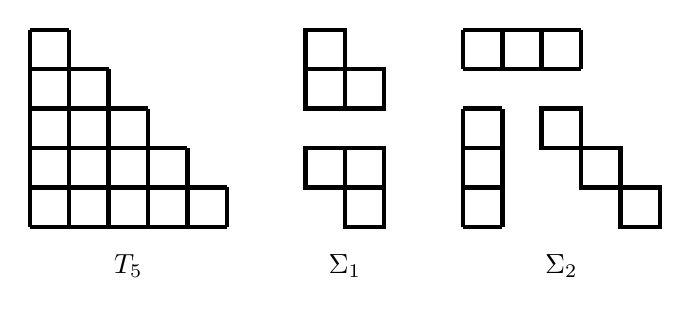
\begin{tikzpicture}

\draw[step=0.5cm,ultra thick] (0,0) grid (5/2,1/2);
\draw[step=0.5cm,ultra thick] (0,1/2) grid (4/2,2/2);
\draw[step=0.5cm,ultra thick] (0,2/2) grid (3/2,3/2);
\draw[step=0.5cm,ultra thick] (0,3/2) grid (2/2,4/2);
\draw[step=0.5cm,ultra thick] (0,4/2) grid (1/2,5/2);
\node[minimum width=1cm] at (5/4,-1/2) {$T_5$};

\draw[ultra thick](7/2,1/2)rectangle(8/2,2/2) ;
\draw[ultra thick](8/2,0/2)rectangle(9/2,1/2) ;
\draw[ultra thick](8/2,1/2)rectangle(9/2,2/2) ;

\draw[ultra thick](7/2,3/2)rectangle(8/2,4/2) ;
\draw[ultra thick](8/2,3/2)rectangle(9/2,4/2) ;
\draw[ultra thick](7/2,4/2)rectangle(8/2,5/2) ;
\node[minimum width=1cm] at (8/2,-1/2) {$\Sigma_1$};

\draw[step=0.5cm,ultra thick] (11/2,0) grid (12/2,3/2);
\draw[step=0.5cm,ultra thick] (11/2,4/2) grid (14/2,5/2);
\draw[ultra thick](13/2,2/2)rectangle(14/2,3/2) ;
\draw[ultra thick](14/2,1/2)rectangle(15/2,2/2) ;
\draw[ultra thick](15/2,0/2)rectangle(16/2,1/2) ;
\node[minimum width=1cm] at (13/2+1/4,-1/2) {$\Sigma_2$};
\draw[ultra thick] (11/2,0)--(11/2,3/2);
\draw[ultra thick] (11/2,4/2)--(11/2,5/2);
\draw[ultra thick] (11/2,4/2)--(14/2,4/2);

\end{tikzpicture}
\caption{\emph{stepenice} $T_5$, skupovi pločica $\Sigma_1$ i $\Sigma_2$}
\label{fig:6}
\end{figure}

\subsection{Kombinatorni rub i karakteristična grupa}
Kod područja ili pločice, ono što zapravo određuje njihova relevantna geometrijska svojstva je njihov rub. Intuitivno je jasno što je obilazak ruba nekog područja. Zato definiramo \emph{orijentirani rub} područja $R$ s početkom u točki $e$ kao obilazak ruba $R$ počevši u $e$ u smjeru suprotnom od kazaljke na satu i označavamo s $\partial R(e)$. Primijetimo, svaki takav obilazak (u pravokutnom slučaju) mogli bismo opisati nizom naredbi \emph{gore}, \emph{dolje}, \emph{lije\-vo} i \emph{desno}. To nam daje ideju obilaske kodirati znakovima pa definiramo slobodnu grupu $F = \langle A,U \rangle$ (od eng.\ \textsl{\textbf{a}cross}, \textsl{\textbf{u}p}), pri čemu će $U$ simbolizirati \emph{gore}, a $A$ \emph{desno}. Uz konvenciju čitanja zdesna nalijevo, orijentirani rub od $T_N$ s početkom u donjem lijevom kutu (v.\ sliku~\ref{fig:6}) odgovarao bi $A^NU^{-N}(A^{-1}U)^N \in F$. Sada možemo orijentirani rub poistovjetiti s elementom grupe $F$.

Vidimo da bi taj element ovisio o početnoj točki, no ona nije suštinski bitna. Štoviše, takvi obilasci su u jednostavnom odnosu --- da dobijemo obilazak koji počinje u nekoj drugoj točki, neki početni dio morali bismo maknuti s početka i dodati na kraj, što u terminima grupe odgovara konjugaciji elementa. Zato definiramo sljedeće pojmove.
\begin{definicija}
\emph{Kombinatorni rub} područja $R$ s oznakom $[\partial R]$ definira se kao konjugacijska klasa (bilo kojeg) orijentiranog ruba $\partial R(e)$ u $F$, odnosno
\[
[\partial R] = \{ W \partial R(e) W^{-1}  \mid W \in F\}.
\]
\end{definicija}
\begin{definicija}
\emph{Karakteristična grupa} skupa pločica $\Sigma$ u oznaci $T(\Sigma)$ je najmanja normalna pogrupa od $F$ koja sadrži kombinatorne rubove svih elemenata od $\Sigma$, odnosno
\[
T(\Sigma) = \langle W\partial S(e) W^{-1} \mid W \in F, S \in \Sigma\rangle.
\]
\end{definicija}
Sljedeći intuitivni rezultat povezuje ove objekte i samo popločavanje te ga navodimo bez dokaza.
\begin{teorem} \label{grupe:nuzno}
Ako se jednostavno povezano područje $R$ može popločati pločicama iz $\Sigma$, onda je $[\partial R]$ sadržan u $T(\Sigma)$.
\end{teorem}
\noindent Primijetimo da je, jer je grupa $T(\Sigma)$ normalna, tvrdnja ekvivalentna tome da je bilo koji orijentirani rub od $R$ sadržan u $T(\Sigma)$.

\subsection{Jedan posebni Cayleyev graf}
Neka je $F_S$ slobodna grupa i $K \unlhd F_S$ njezina normalna podgrupa. Podgrupa $K$ ima lijepu karakterizaciju pomoću neusmjerenog Cayleyevog grafa $\bar{\mathcal{G}}(F_S/K)$ kvocijentne grupe. Neka je $W = s_k^{\varepsilon_k} s_{k-1}^{\varepsilon_{k-1}} \dotsm s_1^{\varepsilon_1}$ pri čemu su $s_i \in S$ generatori i $\varepsilon_i = \pm 1$ riječ u $F_S$. Njoj možemo na prirodni način pridružiti šetnju na grafu $\bar{\mathcal{G}}(F_S/K)$ na sljedeći način: prvo se nalazimo u vrhu koji odgovara neutralnom elementu, a u koraku $i \geq 1$ prelazimo iz vrha pridruženom $W_i = s_i^{\varepsilon_i} s_{i-1}^{\varepsilon_{i-1}} \dotsm s_1^{\varepsilon_1}$ u $W_{i+1} = s_{i+1}^{\varepsilon_{i+1}} W_i$ preko brida između $W_i$ i $W_{i+1}$ s oznakom $i$. Jasno je onda da vrijedi sljedeća propozicija.

\begin{propozicija}
Za riječ $W\in F_S$ vrijedi $W \in K$ ako i samo ako $W$ na $\bar{\mathcal{G}}(F_S/K)$ inducira zatvorenu šetnju s početkom i krajem u neutralnom elementu.
\end{propozicija}
\noindent To nam daje ideju definiranja u suptonom smjeru. Naime, za dani graf $\mathcal{G}$ definiramo skup svih riječi u $F_S$ koje imaju svojstvo da induciraju zatvorenu šetnju oko neutralnog elementa. Uz adekvatni graf taj će skup biti normalna podgrupa, a $\mathcal{G}$ će biti Cayleyev graf kvocijentne grupe.

U našem slučaju, normalna podgrupa $H \unlhd F$ bit će grupa takva da je $\mathcal{G}(F/H)$ na slici~\ref{fig:cayley} Cayleyev graf kvocijente grupe $F/H$. Smatrat ćemo da tamniji bridovi odgovaraju $U$, no zbog simetrije je moguće i suprotno odlučiti. Grupu $H$ moguće je eksplicitno definirati kao najmanju normalnu grupu generiranu s $A^3, U^3$ i $(U^{-1}A)^3$, ali to neće biti od neke važnosti niti koristi. Ključne će biti sljedeće dvije činjenice.
\begin{propozicija} \label{uH}
Kombinatorni rub $[\partial T_N]$ za $N \equiv 0,2 \pmod{3}$ i karakteristične grupe $T(\Sigma_1)$ i $T(\Sigma_2)$ (slika~\ref{fig:6}) nalaze se u $H$.
\end{propozicija}

\begin{figure}[h!]
    \centering
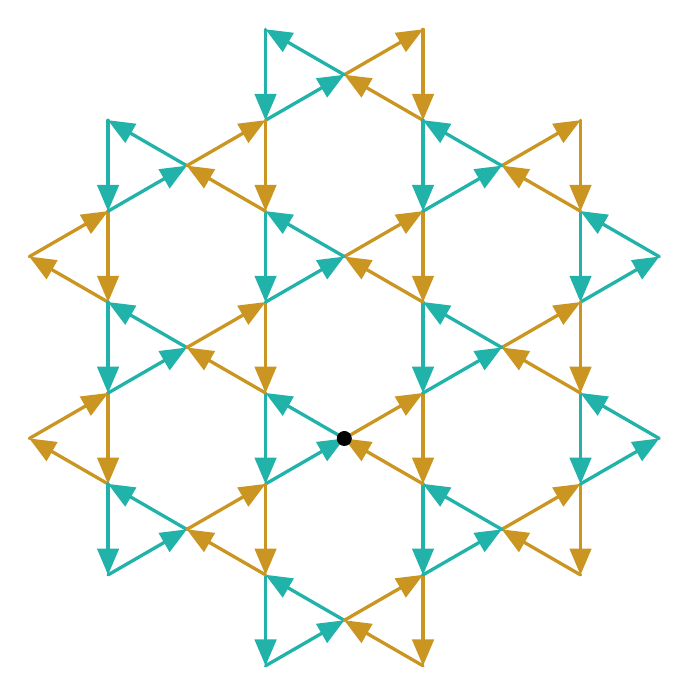
\begin{tikzpicture}[line cap=round,line join=round,>=triangle 45,x=1cm,y=1cm]
\draw [->,line width=1.2pt,color=seagreen] (-3,4.041451884327383) -- (-3,2.88675134594813);
\draw [->,line width=1.2pt,color=seagreen] (-2,3.4641016151377566) -- (-3,4.041451884327383);
\draw [->,line width=1.2pt,color=rawsienna] (-4,2.3094010767585074) -- (-3,2.88675134594813);
\draw [->,line width=1.2pt,color=rawsienna] (-3,2.88675134594813) -- (-3,1.7320508075688776);
\draw [->,line width=1.2pt,color=rawsienna] (-4,0) -- (-3,0.577350269189626);
\draw [->,line width=1.2pt,color=rawsienna] (-3,0.577350269189626) -- (-3,-0.5773502691896251);
\draw [->,line width=1.2pt,color=rawsienna] (-3,-0.5773502691896251) -- (-4,0);
\draw [->,line width=1.2pt,color=seagreen] (-2,-1.1547005383792512) -- (-3,-0.5773502691896251);
\draw [->,line width=1.2pt,color=seagreen] (-3,-0.5773502691896251) -- (-3,-1.7320508075688765);
\draw [->,line width=1.2pt,color=seagreen] (-3,-1.7320508075688765) -- (-2,-1.1547005383792512);
\draw [->,line width=1.2pt,color=seagreen] (0,-2.309401076758503) -- (-1,-1.7320508075688772);
\draw [->,line width=1.2pt,color=seagreen] (-1,-1.7320508075688772) -- (-1,-2.886751345948128);
\draw [->,line width=1.2pt,color=seagreen] (-1,-2.886751345948128) -- (0,-2.309401076758503);
\draw [->,line width=1.2pt,color=rawsienna] (0,-2.309401076758503) -- (1,-1.7320508075688772);
\draw [->,line width=1.2pt,color=rawsienna] (1,-1.7320508075688772) -- (1,-2.8867513459481287);
\draw [->,line width=1.2pt,color=rawsienna] (1,-2.8867513459481287) -- (0,-2.309401076758503);
\draw [->,line width=1.2pt,color=rawsienna] (2,-1.1547005383792526) -- (3,-0.5773502691896268);
\draw [->,line width=1.2pt,color=rawsienna] (3,-0.5773502691896268) -- (3,-1.732050807568879);
\draw [->,line width=1.2pt,color=rawsienna] (3,-1.732050807568879) -- (2,-1.1547005383792526);
\draw [->,line width=1.2pt,color=seagreen] (3,0.5773502691896252) -- (3,-0.5773502691896267);
\draw [->,line width=1.2pt,color=seagreen] (3,-0.5773502691896268) -- (4,0);
\draw [->,line width=1.2pt,color=seagreen] (4,0) -- (3,0.5773502691896252);
\draw [->,line width=1.2pt,color=seagreen] (3,2.8867513459481353) -- (3,1.7320508075688812);
\draw [->,line width=1.2pt,color=seagreen] (3,1.7320508075688812) -- (4,2.309401076758508);
\draw [->,line width=1.2pt,color=seagreen] (4,2.309401076758508) -- (3,2.8867513459481353);
\draw [->,line width=1.2pt,color=rawsienna] (2,3.4641016151377606) -- (3,4.0414518843273886);
\draw [->,line width=1.2pt,color=rawsienna] (3,4.0414518843273886) -- (3,2.8867513459481353);
\draw [->,line width=1.2pt,color=rawsienna] (3,2.8867513459481353) -- (2,3.4641016151377606);
\draw [->,line width=1.2pt,color=rawsienna] (0,4.61880215351701) -- (1,5.196152422706635);
\draw [->,line width=1.2pt,color=rawsienna] (1,5.196152422706635) -- (1,4.041451884327382);
\draw [->,line width=1.2pt,color=rawsienna] (1,4.041451884327382) -- (0,4.61880215351701);
\draw [->,line width=1.2pt,color=seagreen] (-1,4.041451884327385) -- (0,4.61880215351701);
\draw [->,line width=1.2pt,color=seagreen] (0,4.61880215351701) -- (-1,5.196152422706636);
\draw [->,line width=1.2pt,color=seagreen] (-1,5.196152422706636) -- (-1,4.041451884327385);
\draw [->,line width=1.2pt,color=seagreen] (1,-0.577350269189626) -- (1,-1.7320508075688772);
\draw [->,line width=1.2pt,color=rawsienna] (1,-0.577350269189626) -- (0,0);
\draw [->,line width=1.2pt,color=seagreen] (-1,-0.5773502691896256) -- (0,0);
\draw [->,line width=1.2pt,color=rawsienna] (-1,-0.5773502691896256) -- (-1,-1.7320508075688772);
\draw [->,line width=1.2pt,color=seagreen] (-1,0.5773502691896258) -- (-1,-0.5773502691896256);
\draw [->,line width=1.2pt,color=rawsienna] (-2,-1.1547005383792512) -- (-1,-0.5773502691896256);
\draw [->,line width=1.2pt,color=seagreen] (-3,0.577350269189626) -- (-2,1.1547005383792515);
\draw [->,line width=1.2pt,color=rawsienna] (-1,0.5773502691896258) -- (-2,1.1547005383792515);
\draw [->,line width=1.2pt,color=seagreen] (-2,1.1547005383792515) -- (-3,1.7320508075688776);
\draw [->,line width=1.2pt,color=rawsienna] (-2,1.1547005383792515) -- (-1,1.732050807568878);
\draw [->,line width=1.2pt,color=seagreen] (-1,2.886751345948131) -- (-1,1.732050807568878);
\draw [->,line width=1.2pt,color=rawsienna] (-1,2.886751345948131) -- (-2,3.4641016151377566);
\draw [->,line width=1.2pt,color=rawsienna] (-1,4.041451884327385) -- (-1,2.886751345948131);
\draw [->,line width=1.2pt,color=rawsienna] (-1,1.732050807568878) -- (-1,0.5773502691896257);
\draw [->,line width=1.2pt,color=seagreen] (1,4.041451884327382) -- (1,2.8867513459481327);
\draw [->,line width=1.2pt,color=rawsienna] (1,2.8867513459481327) -- (1,1.7320508075688774);
\draw [->,line width=1.2pt,color=seagreen] (1,1.7320508075688774) -- (1,0.5773502691896264);
\draw [->,line width=1.2pt,color=rawsienna] (1,0.5773502691896263) -- (1,-0.5773502691896261);
\draw [->,line width=1.2pt,color=seagreen] (-3,2.88675134594813) -- (-2,3.4641016151377566);
\draw [->,line width=1.2pt,color=rawsienna] (-2,3.4641016151377566) -- (-1,4.041451884327385);
\draw [->,line width=1.2pt,color=seagreen] (-1,1.732050807568878) -- (0,2.309401076758503);
\draw [->,line width=1.2pt,color=rawsienna] (0,2.309401076758503) -- (1,2.8867513459481327);
\draw [->,line width=1.2pt,color=seagreen] (1,2.8867513459481327) -- (2,3.4641016151377606);
\draw [->,line width=1.2pt,color=rawsienna] (0,0) -- (1,0.5773502691896263);
\draw [->,line width=1.2pt,color=seagreen] (1,0.5773502691896263) -- (2,1.1547005383792521);
\draw [->,line width=1.2pt,color=rawsienna] (2,1.1547005383792521) -- (3,1.7320508075688812);
\draw [->,line width=1.2pt,color=seagreen] (2,-1.1547005383792526) -- (1,-0.577350269189626);
\draw [->,line width=1.2pt,color=seagreen] (0,0) -- (-1,0.5773502691896258);
\draw [->,line width=1.2pt,color=rawsienna] (-3,1.7320508075688776) -- (-4,2.3094010767585074);
\draw [->,line width=1.2pt,color=rawsienna] (-1,-1.7320508075688772) -- (-2,-1.1547005383792512);
\draw [->,line width=1.2pt,color=rawsienna] (3,0.5773502691896252) -- (2,1.1547005383792521);
\draw [->,line width=1.2pt,color=seagreen] (2,1.1547005383792521) -- (1,1.7320508075688774);
\draw [->,line width=1.2pt,color=rawsienna] (1,1.7320508075688774) -- (0,2.309401076758503);
\draw [->,line width=1.2pt,color=seagreen] (0,2.309401076758503) -- (-1,2.886751345948131);
\draw [->,line width=1.2pt,color=seagreen] (-3,1.7320508075688776) -- (-3,0.577350269189626);
\draw [->,line width=1.2pt,color=seagreen] (2,3.4641016151377606) -- (1,4.041451884327382);
\draw [->,line width=1.2pt,color=rawsienna] (3,1.7320508075688812) -- (3,0.5773502691896253);
\draw [->,line width=1.2pt,color=seagreen] (1,-1.7320508075688772) -- (2,-1.1547005383792526);
\begin{scriptsize}
\draw [fill=black] (0,0) circle (2.5pt);
\end{scriptsize}
\end{tikzpicture}
    %\includegraphics[width=0.5\textwidth]{cayley.png}
    \caption{Cayleyev graf $\mathcal{G}(F/H)$}
    \label{fig:cayley}
\end{figure}



Druga činjenica je da je graf $\mathcal{G}(F/H)$ planaran. Zbog toga možemo računati indekse zatvorenih šetnji po grafu (kao krivulja) u odnosu na njegove šesterokutne ili trokutaste ćelije (odnosno neke unutarnje točke). Podsjetimo se, za ćeliju $s$ i unutarnju točku $x_s$ indeks puta (zatvorene krivulje) $P$ u odnosu na $s$ u oznaci $\nu(P, s)$ jednak je broju puta koliko se krivulja $P$ omotava oko $s$ u smjeru suprotnom od kazaljke na satu i dan je s
\[
\nu(P,s) = \frac 1{2\pi i} \int_P \frac{\D z}{z - x_s}.
\]
On je neovisan o odabiru točke $x_s$ i aditivan u smislu da za dvije zatvorene krivulje $P_1$ i $P_2$ oko iste točke vrijedi
\begin{equation} \label{aditivnost}
\nu(P_2 P_1, s) = \nu(P_2, s) + \nu(P_1, s).
\end{equation}

Zanimaju nas indeksi zatvorenih šetnji po grafu. Definiramo preslikavanje
\[
\nu(\cdot, s)\colon H\to\mathbb{Z}
\]
tako da riječi $W\in H$ pridruži $\nu(P(W),s)$, gdje je $P(W)$ šetnja inducirana riječju $W$ na način opisan u prijašnjoj diskusiji. Jednakost~\eqref{aditivnost} osigurava da je ovo preslikavanje homomorfizam grupe $H$ i aditivne grupe $(\mathbb{Z},+)$. Slično preslikavanje možemo definirati na većem skupu ćelija $S$:
\[
\nu(P, S) = \sum \limits_{s \in S} \nu(P, s).
\]
Izraz je dobro definiran i očito je $\nu(\cdot,S)\colon H \rightarrow \mathbb{Z}$ opet homomorfizam grupa.

\subsection{Rješenja}
Sada smo spremni dati rješenje problema kojeg smo dali na početku odjeljka. Dakle, govorimo o popločavanju područja $T_N$ pločicama iz skupova $\Sigma_1$ i $\Sigma_2$ sa slike~\ref{fig:6}. 

\begin{teorem} \label{teorem:grupe1}
Popločavanje područja $T_N$ s pločicama iz skupa $\Sigma_1$ (bez rotacija) moguće je ako i samo ako je
\begin{equation} \label{prvi:nuzno}
N \equiv 0, 2, 9, 11 \pmod{12}.
\end{equation}
\end{teorem}

\begin{proof}
Dokazat ćemo samo da je uvjet~\eqref{prvi:nuzno} nužan. Da bi se područje $T_N$ površine $N(N+1)/2$ pokrilo pločicama površine $3$, odmah je nužno 
\begin{equation}\label{02mod3}
N \equiv 0,2 \pmod{3},
\end{equation}
što znači da su zadovoljeni uvjeti propozicije~\ref{uH}. Neka je homomorfizam \[\varphi\colon H\to \mathbb{Z}\] definiran sa 
\[\varphi(W) = \nu(W, S), \quad W \in H,\]
pri čemu je $S$ skup svih šesterokutnih ćelija u Cayleyevom grafu $\mathcal{G}(F/H)$. Primijetimo da je taj homomorfizam (i svaki $H \to \mathbb{Z}$ homomorfizam) invarijantan na konjugacije:
\[
\varphi(hWh^{-1}) = \varphi(h) + \varphi(W) - \varphi(h) = \varphi(W),
\]
pa je $\varphi$ invarijatan na kombinatornim rubovima. Gornju pločicu na slici~\ref{fig:6} označimo sa $S_1$, a donju sa $S_2$. Možemo ustanoviti da vrijedi (pomoću slike~\ref{fig:cayley}, primjeri orijentiranih rubova su $U^{-2}(A^{-1}U)^2A^2$ za $S_1$, $U^2(AU^{-1})^2A^{-2}$ za $S_2$ i $A^NU^{-N}(A^{-1}U)^N$ za $T_N$)
\begin{equation}\label{fiS}
\begin{aligned}
&\varphi[\partial S_1] = 1, \\ 
&\varphi[\partial S_2] = -1 \quad \text i \\ 
\end{aligned}
\end{equation}

\begin{equation}\label{fiT_N}
\varphi[\partial T_N] = \left\lfloor  \frac{N+1}{3} \right\rfloor.
\end{equation}

Po teoremu~\ref{grupe:nuzno} nužno je da se neki orijentirani rub $\partial T_N$ nalazi u $T(\Sigma_1)$, dakle da postoje $m \in \mathbb{N}$, riječi $W_1,\ldots,W_m \in F$, indeksi $k_1,\ldots,k_m \in \{1,2\}$ i predznaci $\varepsilon_1,\ldots,\varepsilon_m = \pm 1$ takvi da
\[
\partial T_N = \prod \limits_{i = 1}^m W_i (\partial S_{k_i})^{\varepsilon_i} W_i^{-1},
\]
pri čemu su $\partial S_i$ opet proizvoljni orijentirani rubovi. Primjenom $\varphi$ s obje strane je
\begin{equation} \label{fimod2}
\varphi [\partial T_N] = \sum \limits_{i=1}^m \varphi\Bigl( W_i (\partial S_{k_i})^{\varepsilon_i} W_i^{-1} \Bigr)
= \sum \limits_{i=1}^m \varepsilon_i \varphi[\partial S_{k_i}] \equiv m\pmod{2},
\end{equation}
pri čemu kongruencija vrijedi zbog $\varepsilon_i = \pm 1$ i~\eqref{fiS}. 

Sada definiramo homomorfizam $\psi\colon H\to \mathbb{Z}$ takav da, shvaćajući $W\in H$ kao šetnju u $\mathbb{R}^2$, vraća broj obilazaka jediničnih kvadratića u smjeru suprotnom kazaljki na satu. Riječ je, dakle, o broju polja opisanog lika pa je $\psi[\partial S_1] = \psi[\partial S_2] = 3$ i
\begin{equation}\label{psiT_N}
\psi[\partial T_N] = \frac{N(N+1)}2.
\end{equation}
Analogno kao u~\eqref{fimod2} dobivamo
\begin{equation}\label{psimod2}
\psi[\partial T_N] \equiv m \pmod{2}.
\end{equation}
Kombinacijom~\eqref{fiT_N},~\eqref{fimod2},~\eqref{psiT_N}~i~\eqref{psimod2} je
\begin{equation} \label{kong}
\left\lfloor  \frac{N+1}{3} \right\rfloor \equiv \frac{N(N+1)}2 \pmod{2}.
\end{equation}
Pokaže se da je~\eqref{02mod3}~i~\eqref{kong} ekvivalentno s~\eqref{prvi:nuzno}.
\end{proof}


\begin{teorem} \label{teorem:grupe2}
Popločavanje područja $T_N$ s pločicama iz skupa $\Sigma_2$ (bez rotacija) nije moguće ni za koji $N$.
\end{teorem}

\begin{proof}
Ponovo vrijedi~\eqref{02mod3}. Neka je homomorfizam \[\varphi_U\colon H\to \mathbb{Z}\] definiran sa 
\[\varphi_U(W) = \nu(W, S_U), \quad W \in H,\]
pri čemu je $S_U$ skup svih trokutastih ćelija s bridovima $U$ (tamni na slici~\ref{fig:cayley}) u Cayleyevom grafu $\mathcal{G}(F/H)$. Na slici~\eqref{fig:6} označimo horizontalnu pločicu s $S_3$, vertikalnu s $S_4$ i dijagonalnu s $S_5$. Pokazuje se da vrijedi

\begin{gather}
\varphi_U [\partial S_3] = \varphi_U[\partial S_4] = \varphi_U[\partial S_5] = 0 \quad \text i \label{fiUnule}\\ 
\varphi_U [\partial T_N] = \left\lfloor  \frac{N+1}{3} \right\rfloor. \label{fiUT_N}
\end{gather}
Ponovo je po teoremu~\ref{grupe:nuzno} nužno da se neki orijentirani rub $\partial T_N$ nalazi u $T(\Sigma_2)$, dakle da postoje $m \in \mathbb{N}$, riječi $W_1,\ldots,W_m \in F$, indeksi $k_1,\ldots,k_m \in \{3,4,5\}$ i predznaci $\varepsilon_1,\ldots,\varepsilon_m = \pm 1$ takvi da
\[
\partial T_N = \prod \limits_{i = 1}^m W_i (\partial S_{k_i})^{\varepsilon_i} W_i^{-1},
\]
pri čemu su $\partial S_i$ opet proizvoljni orijentirani rubovi. Primjenom $\varphi_U$ s obje strane je
\begin{equation*}
\varphi_U [\partial T_N] = \sum \limits_{i=1}^m \varphi_U\Bigl( W_i (\partial S_{k_i})^{\varepsilon_i} W_i^{-1} \Bigr)
= \sum \limits_{i=1}^m \varepsilon_i \varphi_U[\partial S_{k_i}] =0,
\end{equation*}
pri čemu treća jednakost vrijedi zbog~\eqref{fiUnule}. Time smo za $N \geq 2$ došli do kontradikcije s~\eqref{fiUT_N}.
\end{proof}

\subsection{Osvrt na bojanja}
Prirodno je pitati se jesmo li tvrdnje teorema mogli dokazati i nekakvim bojanjem ili su ovakve naprednije metode zaista nužne. Odgovor je da dokaz bojanjem zaista nije bio moguć. Štoviše, nije bio moguć ni za dokaz teorema~\ref{walkupteorem}. Ovdje ćemo sasvim ukratko objasniti kako se do takvog rezultata dolazi, a puno opsežnija diskusija i dokazi tvrdnji mogu se naći u~\cite{conway}.

Najprije ćemo definirati svojevrsnu generalizaciju popločavanja i bojanje u punoj općenitosti. 
\begin{definicija}
\emph{$\mathbb{Z}$-popločavanje} područja $R$ pločicama iz $\Sigma$ je popločavanje nekog nadskupa $R' \supseteq R$ u kojemu se pločice smiju preklapati i 
\begin{itemize}
\item svakoj pločici pridružena je težina $1$ ili $-1$,
\item svakom polju područja $R'$ računa se težina na njemu zbrajajući težine pločica koje ga prekrivaju i
\item na svakom polju u $R$ mora biti težina $1$, a na svakom izvan $R$ težina $0$.
\end{itemize}
\end{definicija}
\begin{definicija}
\emph{Opće bojanje} je homomorfizam $\varphi\colon C\to A$ pri čemu je $C\leq F$ podgrupa određena samo onim riječima koje odgovaraju zatvorenim obilascima, a $A$ neka Abelova grupa. \emph{Opći argument bojanjem} je dokaz da popločavanje jednostavno povezanog područja nije moguće jer se $\varphi[\partial R]$ ne nalazi u $\varphi(T(\Sigma))$. 
\end{definicija}
\begin{teorem} \label{sgn}
Svaki opći argument bojanjem koji opovrgava postojanje popločavanja $R$ s pločicama iz $\Sigma$ opovrgava i postojanje $\mathbb{Z}$-popločavanja $R$ pločicama iz $\Sigma$.
\end{teorem}
Teorem~\ref{sgn} zapravo govori da kad god postoji $\mathbb{Z}$-popločavanje, nemogućnost popločavanja neće biti moguće dokazati argumentom bojanja. Slijedi rezultat koji govori da su uvjeti za postojanje $\mathbb{Z}$-popločavanja u uvjetima teorema~\ref{walkupteorem}, teorema~\ref{teorem:grupe1} i teorema~\ref{teorem:grupe2} zaista širi nego za uobičajena popločavanja, što znači da su neke alternativne tehnike dokazivanja doista bile potrebne.
\begin{teorem} Vrijede sljedeći nužni i dovoljni uvjeti za $\mathbb{Z}$-popločavanja.
\begin{enumerate}
\item $\mathbb{Z}$-popločavanje pravokutnika $m \times n$ $T$-pločicama moguće je ako i samo ako $8 \mid mn$.
\item $\mathbb{Z}$-popločavanje $T_N$ pločicama iz $\Sigma_1$ (bez rotacija) moguće je ako i samo ako
\[N \equiv 0,2 \pmod{3}.\]
\item $\mathbb{Z}$-popločavanje $T_N$ pločicama iz $\Sigma_2$ (bez rotacija) moguće je ako i samo ako
\[N \equiv 0,8 \pmod{9}.\]
\end{enumerate}
\end{teorem}





\printbibliography

\end{document}
